\documentclass{article}
\usepackage{amsmath} % For align*
\usepackage{circuitikz} % For circuit diagrams
\usepackage{bookmark} % For links
\usepackage{float} % For the [H] option on figures
\usepackage{graphicx} % For images
\usepackage{tikz} % For diagrams
\usepackage{siunitx} % For units

\graphicspath{{./images/}}
\hypersetup{
  colorlinks=true,
  linkcolor=blue,
  urlcolor=blue
}

\renewcommand{\vec}[1]{\boldsymbol{\mathbf{#1}}}

\begin{document}

\tableofcontents

\section{Introduction}

I recently built this self-balancing inverted pendulum on a cart. If you've ever tried to keep something like a broom or a stick upright on your hand you'll know it can be quite tricky! Gravity's constantly pulling it down, so if it’s not perfectly vertical it’ll start to fall. The same thing happens to the pendulum but the cart's programmed to move left and right in a way that keeps it upright.

In this video I’ll explain how I built this, starting with the math and physics, and then the construction and code. The math will make the most sense if you're familiar with calculus and a little linear algebra but if not, don't worry, you should still be able to follow along.

\section{Equations of Motion}

If we want to control this system we need to know how it behaves when the cart's free to move, so let’s derive its equations of motion. First we need to define our coordinate system and variables in a diagram:

\begin{figure}[h]
  \centering
  \begin{tikzpicture}
    % x
    \draw (-2, 0.3) -- (-2, 0.7);
    \draw[dashed] (-2, 0.5) -- node[above] {$x$} (0, 0.5);

    % Cart
    \draw (0, 0) rectangle node {$m_1$} (2, 1);

    % Pendulum
    \draw (1, 1) -- (0.5, 3);
    \draw[dashed] (1, 1) -- (1, 3);
    \draw (0.37, 3.4) node {$m_2$} circle (0.4cm);

    % l
    \node at (0.5, 1.8) {$l$};

    % Theta
    \draw (1, 2.8) arc (90:117:1);
    \node at (0.8, 2.5) {$\theta$};

    % Axes
\draw[->] (3, 0.5) -- (4, 0.5) node[right] {$x$};
\draw[->] (3, 0.5) -- (3, 1.5) node[above] {$y$};
  \end{tikzpicture}
\end{figure}

We have a cart of mass $m_1$ that can only move along the $x$-axis and its position $x$ is measured from some origin point. The cart is connected to a simple pendulum of length $l$ and mass $m_2$ which is at an angle $\theta$ from vertical.

With that out of the way, now we can determine the Lagrangian of the system which is defined as the difference between its kinetic and potential energies: $\mathcal{L} = T - U$. Well, what are those energies?

Starting with the cart, its kinetic energy is \[T_\text{cart} = \frac{1}{2} m_1 v^2\] but because it can only move along the $x$-axis its velocity has no $y$ component this is equivalent to \[T_\text{cart} = \frac{1}{2} m_1 \dot{x}^2.\] Again, it can't move up or down, so its potential energy can't change and we might as well set it to $0$ \[U_\text{cart} = 0.\]

Next, the pendulum. Because it's joined to the cart its $x$ coordinate changes as cart moves, and both of its coordinates change as it rotates. We can write its coordinates as \begin{align*}
  X & = x - l \sin \theta \\
  Y & = l \cos \theta.
\end{align*} Differentiating these equations with respect to time gives the $x$ and $y$ components of the pendulum's velocity \begin{align*}
  \dot{X} & = \dot{x} - l \dot{\theta} \cos \theta \\
  \dot{Y} & = -l \dot{\theta} \sin \theta.
\end{align*} Using the Pythagorean theorem we can combine these to find the squared magnitude of the pendulum's velocity \begin{align*}
  V^2 & = \dot{X}^2 + \dot{Y}^2                                                      \\
      & = (\dot{x} - l \dot{\theta} \cos \theta)^2 + (-l \dot{\theta} \sin \theta)^2 \\
      & = \dot{x}^2 - 2 l \dot{\theta} \dot{x} \cos \theta + l^2 \dot{\theta}^2
\end{align*}
and we can use this to find its kinetic energy \begin{align*}
T_\text{pendulum} & = \frac{1}{2} m_2 V^2                                                                          \\
                    & = \frac{1}{2} m_2 (\dot{x}^2 - 2 l \dot{\theta} \dot{x} \cos \theta + l^2 \dot{\theta}^2).
\end{align*} Unlike the cart, the pendulum's potential energy can change — as we saw, when it rotates it moves up and down so its gravitational potential energy changes. If we say its potential energy is $0$ when its $y$ coordinate is $0$, then we can define its potential energy to be \begin{align*}
  U_\text{pendulum} & = m_2 g y              \\
                    & = m_2 g l \cos \theta.
\end{align*}

Combining all of those energies gives a Lagrangian of \begin{align*}
  \mathcal{L} & = T - U                                                                                                                                     \\
              & = T_\text{cart} + T_\text{pendulum} - U_\text{cart} - U_\text{pendulum}                                                                     \\
              & = \frac{1}{2} m_1 \dot{x}^2 + \frac{1}{2} m_2 (\dot{x}^2 - 2 l \dot{\theta} \dot{x} \cos \theta + l^2 \dot{\theta}^2) - m_2 g l \cos \theta \\
              & = \frac{1}{2} (m_1 + m_2) \dot{x}^2 + \frac{1}{2} m_2 (l^2 \dot{\theta}^2 - 2 l \dot{\theta} \dot{x} \cos \theta) - m_2 g l \cos \theta.
\end{align*}

Now that we have the Lagrangian we can apply the Euler-Lagrange equation to each of the system's two coordinates $\theta$ and $x$. For $\theta$ we get \begin{align*}
  0 & = \frac{d}{d t} \frac{\partial \mathcal{L}}{\partial \dot{\theta}} - \frac{\partial \mathcal{L}}{\partial \theta}                 \\
    & = \frac{d}{d t} (m_2 l^2 \dot{\theta} - m_2 l \dot{x} \cos \theta) - m_2 l \dot{\theta} \dot{x} \sin \theta - m_2 g l \sin \theta \\
    & = l \ddot{\theta} - \ddot{x} \cos \theta - g \sin \theta
\end{align*} and for $x$ we get \begin{align*}
  0 & = \frac{d}{d t} \frac{\partial L}{\partial \dot{x}} - \frac{\partial \mathcal{L}}{\partial x} \\
    & = \frac{d}{d t} [(m_1 + m_2) \dot{x} - m_2 l \dot{\theta} \cos \theta]                        \\
    & = (m_1 + m_2) \ddot{x} - m_2 l \ddot{\theta} \cos \theta + m_2 l \dot{\theta}^2 \sin \theta.
\end{align*} Rearranging these two equations and solving for $\ddot{\theta}$ and $\ddot{x}$ gives us our equations of motion \begin{align*}
\ddot{\theta} & = \frac{(m_1 + m_2) g \sin \theta - m_2 l \dot{\theta}^2 \cos \theta \sin \theta}{l (m_1 + m_2) - m_2 l \cos^2 \theta} \\
\ddot{x}      & = \frac{m_2 \sin 2 \theta - 2 m_2 l \dot{\theta}^2 \sin \theta}{2 m_1 + m_2 - m_2 \cos 2 \theta}.
\end{align*}

Now that we've got them how do we know they're correct? One way would be to solve them for $\theta$ and $x$ and see if their predictions are reasonable. I certainly don't know how to solve them analytically, but we can solve them numerically. This is a Mathematica notebook I created to do just that. You can see we define some constants like gravity, the length of the pendulum, etc. We define the initial conditions for the simulation — here the pendulum is starting $\ang{30}$ from vertical. We solve the equations of motion numerically, and generate an animation of the solution which you can see if I evaluate the notebook.

The pendulum swings back and forth as we expect, but interestingly it also causes the cart to move. This model doesn't include air resistance or friction so it'll keep swinging forever, but we can tweak the variables and see how that affects the solution. Let's make the cart much heavier. It still moves, but much less than before, which makes sense.

\section{Linearisation}

These equations look good, but they're quite complicated so it might be difficult to analyse the stability of the system and determine how to control it. Can we simplify them at all? Well, one approach is to linearise them.

Linearising a function means finding a linear approximation of it at a particular point. For example, if we graph a function $y = f(x)$ and we want to linearise it at $x = 1$, we evaluate it at the point to find its $y$ coordinate, and we evaluate its derivative at the point to find its slope. Using this information we can plot a new function that passes through the original point and extends its slope in both directions. It's a line. If you zoom in enough the line does a pretty good job of approximating the function. As you move away it doesn't do as good of a job, but if you only care about the area around the point that's fine.

\begin{figure}[H]
  \centering
  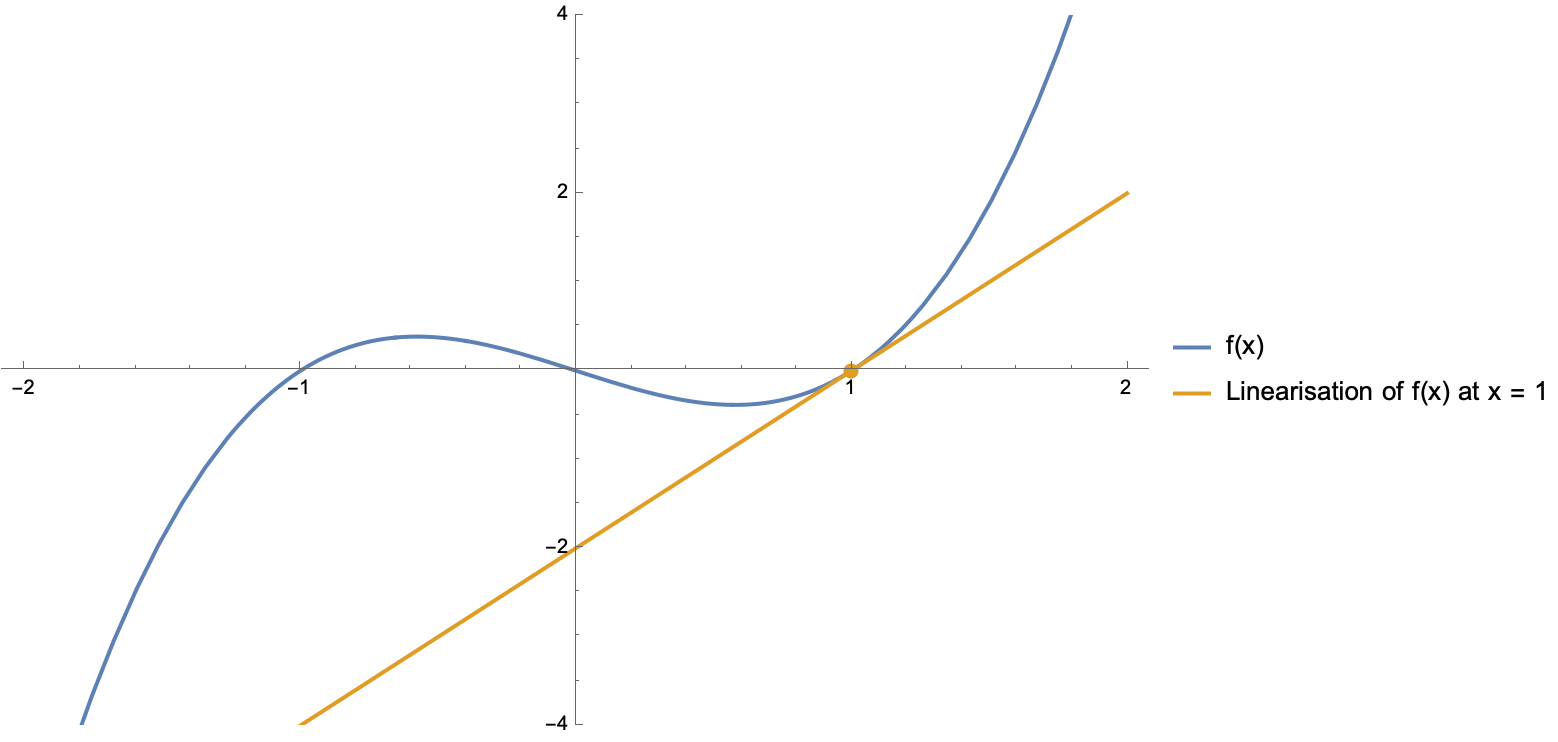
\includegraphics[width=\textwidth]{linearisation1}
\end{figure}

This works in three dimensions too. If we graph another function $z = g(x, y)$ and we want to linearise it at a point, again we evaluate it at the point to find its $z$ coordinate, we evaluate its derivative with respect to $x$ at the point to find its slope in the $x$ direction, and we evaluate its derivative with respect to $y$ at the point to find its slope in the $y$ direction. Using this information we can plot a new function that passes through the original point and extends the slopes in both the $x$ and $y$ directions. It's a plane. Like before, it approximates the function best when you're close to the point and gets worse as you move away.

\begin{figure}[H]
  \centering
  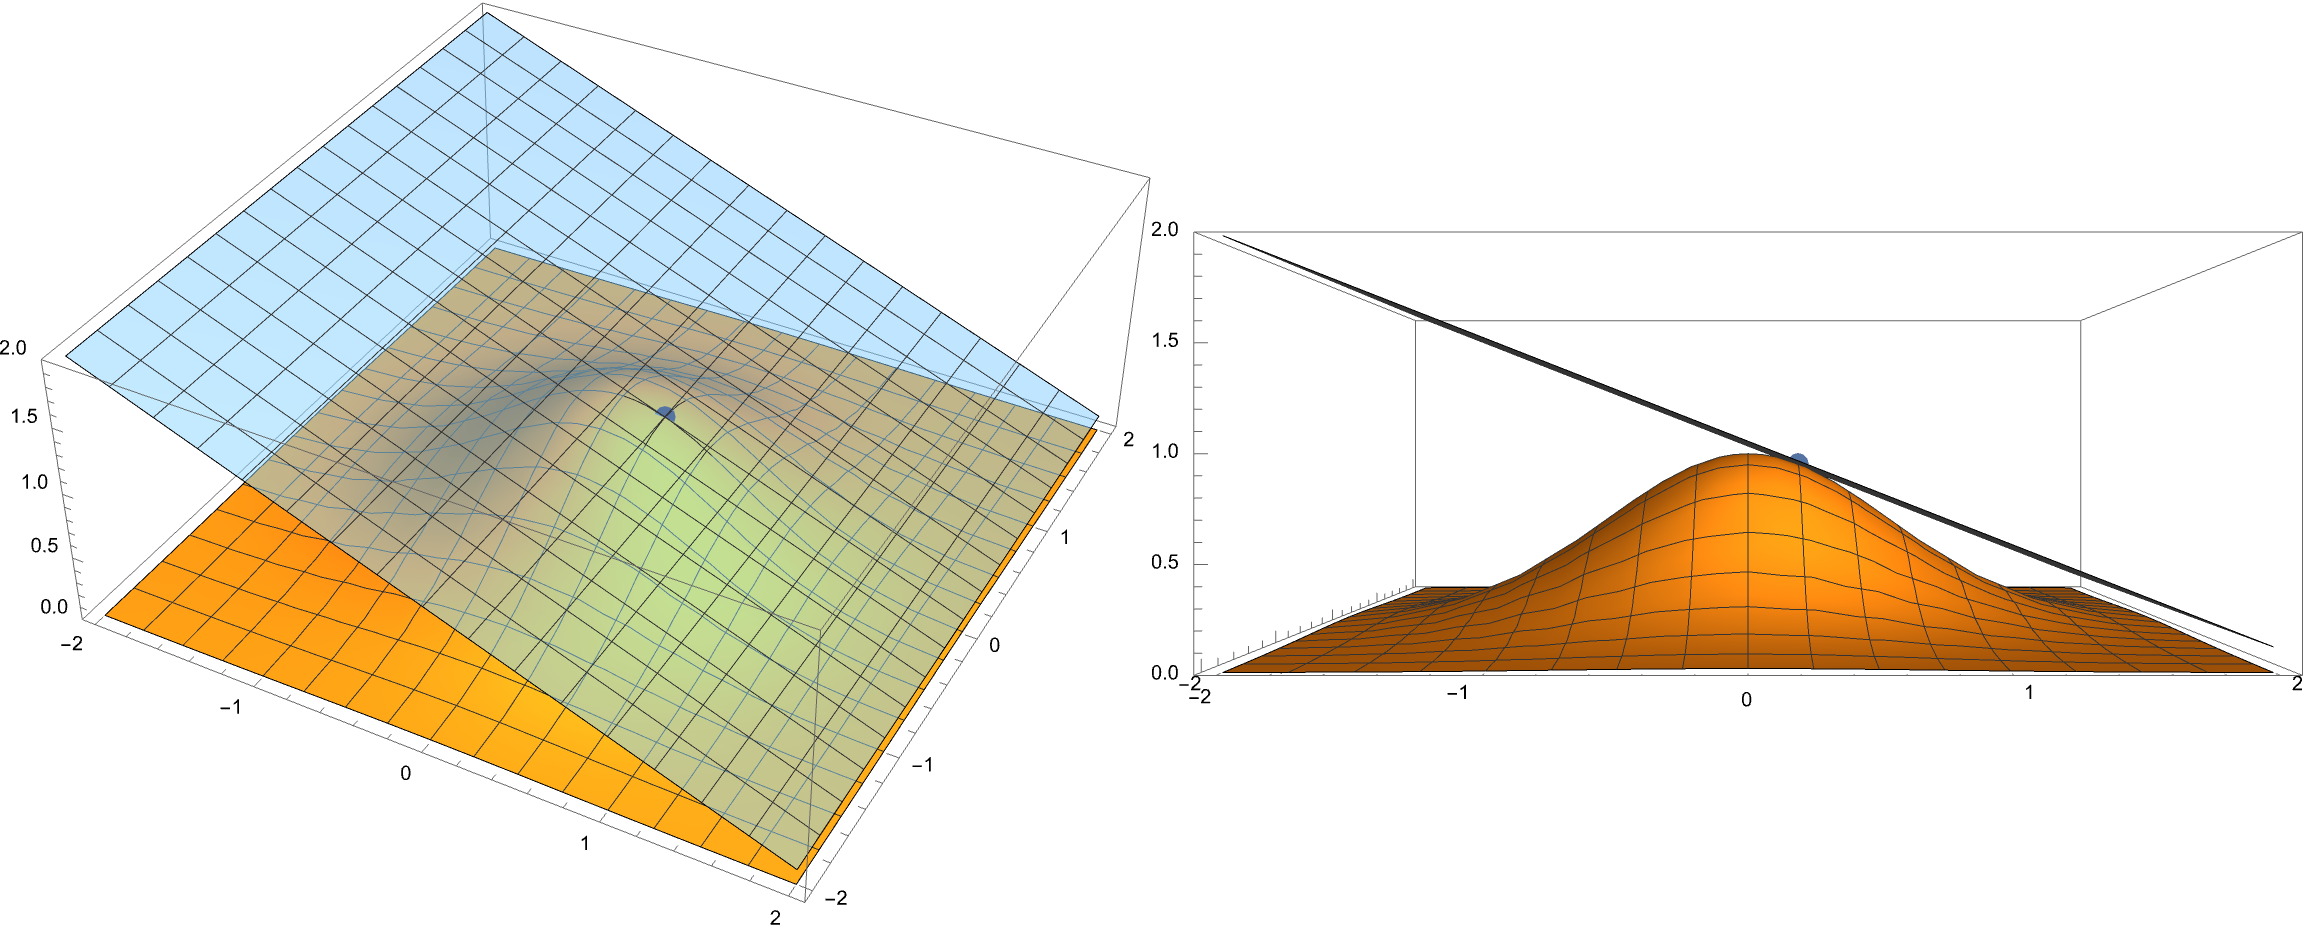
\includegraphics[width=\textwidth]{linearisation2}
\end{figure}

However, something to remember is our goal is to keep the cart in the middle of the track, the pendulum upright, and neither of them moving. In other words, we want all four variables $\theta$, $\dot{\theta}$, $x$, and $\dot{x}$ to be $0$. The further they are from $0$ the less likely it is we'll be able to recover and we might have to accept that the pendulum's going to fall over. It sounds like linearisation might work for us!

So how do we linearise our equations of motion?

\end{document}